\section{Fundamentos de la virtualización}\label{fundamentos}

Para realizar una referencia a los fundamentos teóricos, a continuación, se presentan en primera instancia el concepto mismo de la virtualización, seguido de elementos y técnicas de utilización; además se presenta la  taxonomía de referencias utilizada en el presente trabajo. 

\subsection{Virtualización}

La virtualización puede ser considerada como la combinación de diferentes tecnologías, que ofrece a las organizaciones gran variedad de ventajas como el apoyo para la gestión de grandes volúmenes de datos, la posibilidad de escalar rápidamente la infraestructura de aplicaciones y el aprovechamiento de grandes capacidades de cómputo; técnicamente y según lo señala \textcite{Kusnetzky2011}, la virtualización permite abstraer aplicaciones y los componentes subyacentes de hardware para ser presentados como una vista lógica o virtual de estos recursos \parencite{AbdElRahem2016}. Esta vista lógica puede ser en ocasiones notablemente diferente a la vista física, la cual por lo general se construye a partir del exceso de recursos de computación, tales como el poder de  procesamiento, la memoria, la capacidad de almacenamiento o incluso el ancho de banda \parencite{Stallings2015}.\\

En complemento a lo anterior, \textcite{Silberschatz2014} señalan que la virtualización está relacionada con la tecnología que permite que los sistemas operativos se ejecuten como aplicaciones dentro de otros sistemas operativos. \\

La virtualización también incluye el término \textit{emulación}, el cual es ampliamente conocido y hace referencia al hecho de tener diferencias entre la arquitectura base y la proyectada en el proceso de virtualización.\\

Entre los objetivos de la virtualización se tiene: aumento de los niveles de rendimiento computacional, favorecer la escalabilidad y disponibilidad de sus soluciones tecnológicas de manera eficiente y eficaz, además de propender por unificar y usar de forma fácil las estructuras de administración y seguridad de la infraestructura computacional existente \parencite{Kusnetzky2011, Hui2014}. \\

A través de la virtualización es posible crear una vista lógica  que combine recursos computacionales para presentar uno o varios entornos operativos, esto es por ejemplo, que muchos computadores físicos sean vistos como un único gran recurso (agregación de recursos) o por el contrario, que un solo computador sea visto como múltiples instancias de sí mismo (división de recursos)  \parencite{Silberschatz2014}. La virtualización puede tener lugar usando metodologías como partición o agregación de hardware y software, simulación de máquina parcial o completa, emulación y tiempo compartido entre otros \parencite{Chiueh2005, Hoopes2009}. La partición de recursos es una de las formas más comunes de usar la virtualización, en este caso, es posible agregar la capa de virtualización sobre el recurso real, tal como se muestra en la figura \ref{fig:divisionDeRecursosConVirtualizacion}. Esta capa de virtualización permite que varios recursos virtuales sean ejecutados simultáneamente ubicados sobre un mismo recurso real.

\begin{figure}[!hbtp]
	\centering
	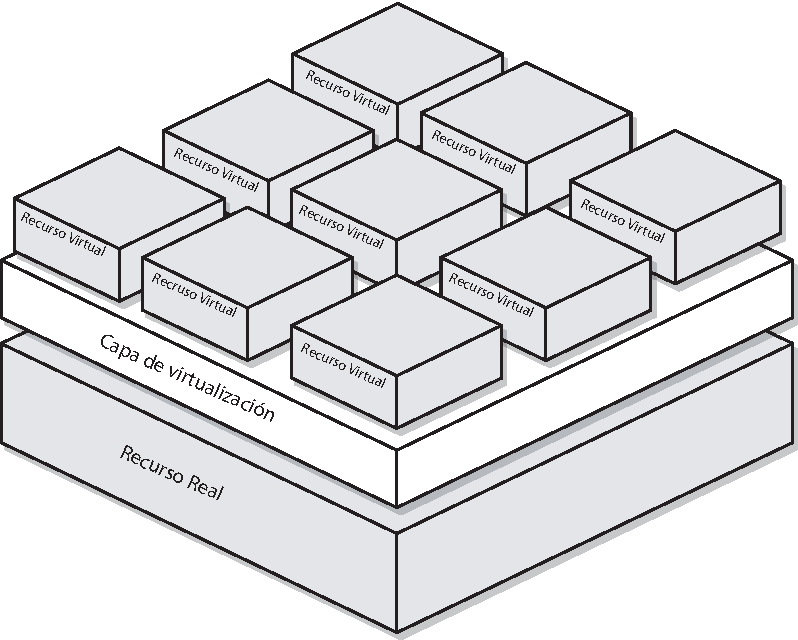
\includegraphics[width=8cm]{Pictures/divisionRecursosFisicosConV12N.pdf}
	\vspace{-0.2cm}
	\caption{División de recursos a través de la virtualización}
	\label{fig:divisionDeRecursosConVirtualizacion}
\end{figure}

Desafortunadamente la arquitectura de computadores x86 a pesar de ser una de las más populares en el mundo, no es virtualizable al 100\% \parencite{Adams}. En esta arquitectura, al ejecutar instrucciones en modo no privilegiado, algunas de ellas pueden fallar silenciosamente en lugar de provocar una trampa y así brindar su respectivo tratamiento. Esta situación ha tenido respuesta a través de mecanismos y formas de virtualización que actúan en diversos niveles de abstracción. Los niveles de abstracción dónde la virtualización tiene lugar son los siguientes: nivel del conjunto de instrucciones, nivel de abstracción de hardware, nivel de sistema operativo, nivel de interfaz de biblioteca de nivel de usuario y finalmente en el nivel de aplicación \parencite{Chiueh2005}.\\

Los conceptos acerca de la virtualización se presentan agrupados en las categorías \textit{elementos} y  \textit{técnicas de la virtualización}, cuya descripción se muestra en los apartados siguientes.


\subsection{Elementos de la virtualización}

Los elementos \textit{máquina real}, \textit{máquina virtual} y \textit{monitor de máquinas virtuales}, son considerados básicos para la comprensión de las tecnologías de virtualización y se describen a continuación.

\subsubsection{Máquina real}

El término \textit{máquina real} (RM por sus siglas en inglés \textit{Real Machine}) referencia los elementos físicos de la infraestructura tecnológica que conforman un computador; ya sea un computador personal, una estación de trabajo o un servidor. Otras referencias a este concepto son los términos en inglés \textit{hardware}, \textit{physical hardware}, \textit{bare-metal}. En el ámbito informático comercial es común que se refiera al concepto de RM utilizando la palabra \textit{anfitrión} o en inglés \textit{host} \parencite{VMware2008}. 

\subsubsection{Máquina virtual}

El concepto de \textit{máquina virtual} (VM por sus siglas en inglés \textit{Virtual Machine}) no es nuevo y fue formalizado en la tesis de  \textcite{Goldberg1973} y publicado en el trabajo académico de \textcite{Goldberg1974}; en estos trabajos se establecen las bases conceptuales para determinar el significado de una VM, siendo esta asumida como un duplicado eficiente y aislado de una RM, ver figura \ref{fig:TheVirtualMachineMonitor_Popek1974}.\\

Actualmente el concepto de VM hace referencia a un ambiente operativo para el conjunto de aplicaciones del nivel de usuario, lo cual incluye librerías, llamados al sistema, interfaces/servicios, configuraciones del sistema, procesos y archivos de estado \parencite{Chiueh2005}. Otra forma de presentar el concepto de VM según \textcite{Solis2014}, es relacionarlo con una capa de software, la cual se posiciona entre los recursos hardware o software y las aplicaciones. También es muy común que en el ámbito informático comercial se refiera al concepto de VM utilizando la palabra \textit{invitado(a)} o en inglés \textit{guest} \parencite{VMware2008}. Finalmente, \textcite{Pek2013} establecen que una VM, es también considerada como una abstracción de recursos de computación presentados como servicio para permitir que éstos operen simultáneamente sobre la misma infraestructura de la RM .

\begin{figure}[!hbtp]
	\centering
	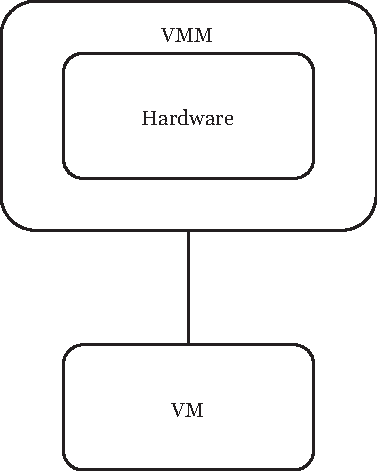
\includegraphics[width=5cm]{Pictures/VMMPopek1974.pdf}
	\vspace{-0.2cm}
	\caption{Visión general de MV y VMM por \textit{Popek} y \textit{Goldberg}.\footnotemark[2]{} }
	\label{fig:TheVirtualMachineMonitor_Popek1974}
\end{figure}

\footnotetext[2]{Basada en la figura original del monitor de máquina virtual del trabajo \textit{formal Requirements for Virtualizable Thrid Generation Architectures} de Gerald J. Popek y Robert P. Goldberg en 1974.}

\subsubsection{Monitor de máquinas virtuales}

El término monitor de máquina virtual (VMM por sus siglas en inglés \textit{Virtual Machine Monitor}), fue establecido en el trabajo de \textit{Popek} y \textit{Goldger} \cite{Popek1974}, en el cual  se definieron las bases conceptuales de un VMM como una pieza de software que tiene las siguientes tres características esenciales: 
\begin{enumerate}
	\item \textit{Equivalencia}: Proveer un ambiente para los programas, el cual es idéntico a la máquina original.\\
	
	\item \textit{Desempeño}: Los programas que se ejecutan en este ambiente muestran, en el peor de los casos, solo una degradación en velocidad.\\
	
	\item \textit{Control de recursos}: El VMM está en completo control de los recursos del sistema.\\ 
\end{enumerate}

La definición de un VMM está relacionada con una capa software que proporciona  infraestructura de soporte utilizando los recursos de un nivel más bajo (generalmente \textit{hardware}), para crear múltiples máquinas virtuales que son independientes y aisladas entre sí \parencite{Chiueh2005, Cafaro2011}. De manera similar, \textcite{Stallings2015}  determina  que un VMM, es un software que actúa como un intermediador entre la RM y las VMs; este software es comúnmente llamado \textit{hipervisor}, el cual permite que muchas máquinas virtuales coexistan de forma segura en una única RM. La cantidad de máquinas virtuales que existen en una sola máquina real, determina el índice de consolidación que para el caso particular de la figura \ref{fig:VMM}, es de 9 a 1 expresado como (9:1). Entre mayor sea el índice de consolidación mejor será el ROI y menos el TCO de la máquina real utilizada. Algunas de las funciones y responsabilidades de los hipervisores son la emulación, aislamiento, asignación de recursos y el encapsulamiento \parencite{Hoopes2009}.

\begin{figure}[!hbtp]
	\centering
	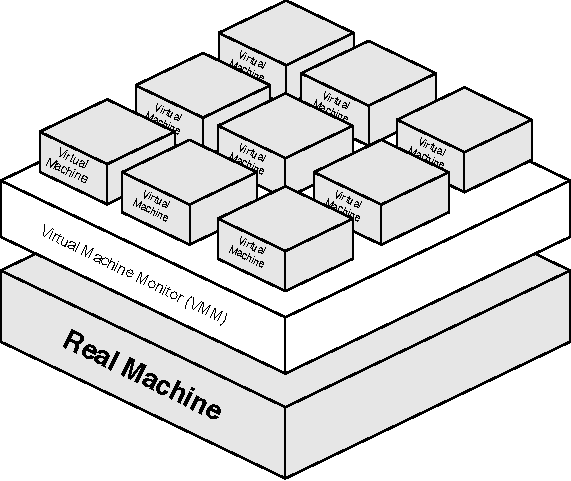
\includegraphics[width=8cm]{Pictures/VMMGeneric.pdf}
	\vspace{-0.2cm}
	\caption{Monitor de máquinas virtuales (VMM) o hipervisor}
	\label{fig:VMM}
\end{figure}

\subsection{Técnicas de virtualización}

A continuación, se describen dos de las principales técnicas de virtualización comúnmente utilizadas con son la \textit{basada en hipersivor} y la \textit{basada en contenedores}, estas técnicas permiten en general lograr consolidar componentes hardware y brindar un ambiente de ejecución virtual para sistemas o procesos respectivamente.

\subsubsection{Virtualización basada en hipervisor}

La técnica de virtualización basada en hipervisor consiste en la utilización del VMM como elemento central, el cual puede estar ubicado de dos maneras diferentes. La primera forma consiste en ubicar el hipervisor directamente sobre el hardware. Esta técnica es también conocida como virtualización \textit{bare-metal} o \textit{nativa}, y al hipervisor se le denomina de \textit{Tipo 1} (Figura \ref{fig:Bare-metalHypervisor}).  La utilización de este tipo de hipervisor no necesita la presencia de un sistema operativo subyacente en la RM. La segunda realiza la instalación del hipervisor sobre un sistema operativo existente. Esta técnica es también conocida como virtualización \textit{alojada} o \textit{basada en host}, y al hipervisor se le considera de \textit{Tipo 2} (ver figura \ref{fig:host-basedHypervisor}). Como característica general de la virtualización basada en hipervisor, se tiene la creación de máquinas virtuales completas, las cuales pueden ejecutar sistemas operativos \textit{guest} independientes y posiblemente diferentes, siempre y cuando sean compatibles con arquitectura virtual entregada. 


\begin{figure}[!hbtp]
	\centering
	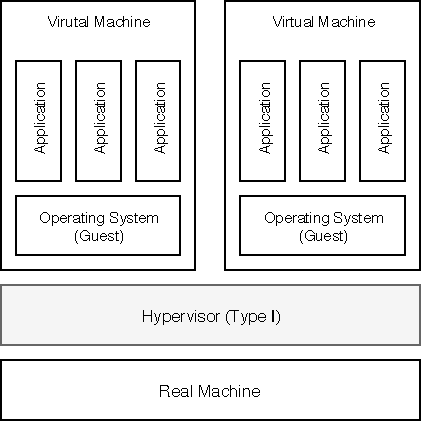
\includegraphics[width=8cm]{Pictures/bare-metalHypervisor.pdf}
	\vspace{-0.2cm}
	\caption{Bare-metal Hypervisor}
	\label{fig:Bare-metalHypervisor}
\end{figure}

\begin{figure}[ht] %[!hbtp]
	\centering
	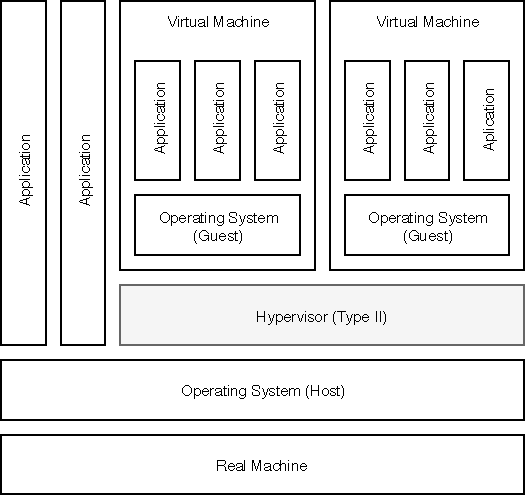
\includegraphics[width=8cm]{Pictures/host-basedHypervisor.pdf}
	\vspace{-0.2cm}
	\caption{Hoste based hypervisor}
	\label{fig:host-basedHypervisor}
\end{figure}

\subsubsection{Virtualización basada en contenedores}

La técnica de virtualización basada en contenedores utiliza como base un sistema operativo preexistente y consiste en la generación de entornos virtuales de ejecución para procesos. Estos entornos de ejecución son comúnmente llamados \textit{contenedores} (ver figura \ref{fig:container-baseVirtualization}). Esta técnica de virtualización gana cada día mayor aceptación en los ámbitos académico y productivo, debido a que, a diferencia de la virtualización basada en hipervisor, no es necesario generar VMs con sistemas operativos completos, sino que se utilizan partes fundamentales del sistema operativo \textit{host} para generar los entornos virtuales de operación para los procesos \parencite{Kon2017}. Lo anterior supone una menor carga computacional necesaria para generar el entorno virtual y de igual forma supone que dicho entorno está sujeto al tipo de sistema operativo subyacente. 


\begin{figure}[ht] % [!hbtp]
	\centering
	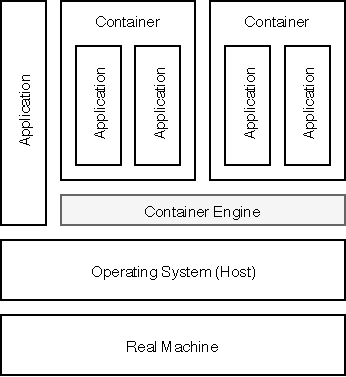
\includegraphics[width=8cm]{Pictures/container-baseVirtualization.pdf}
	\vspace{-0.2cm}
	\caption{Container-based virtualization}
	\label{fig:container-baseVirtualization}
\end{figure}


\subsection{Taxonomía de Tecnologías de Virtualización}



\begin{figure}[!htp]
	\centering
	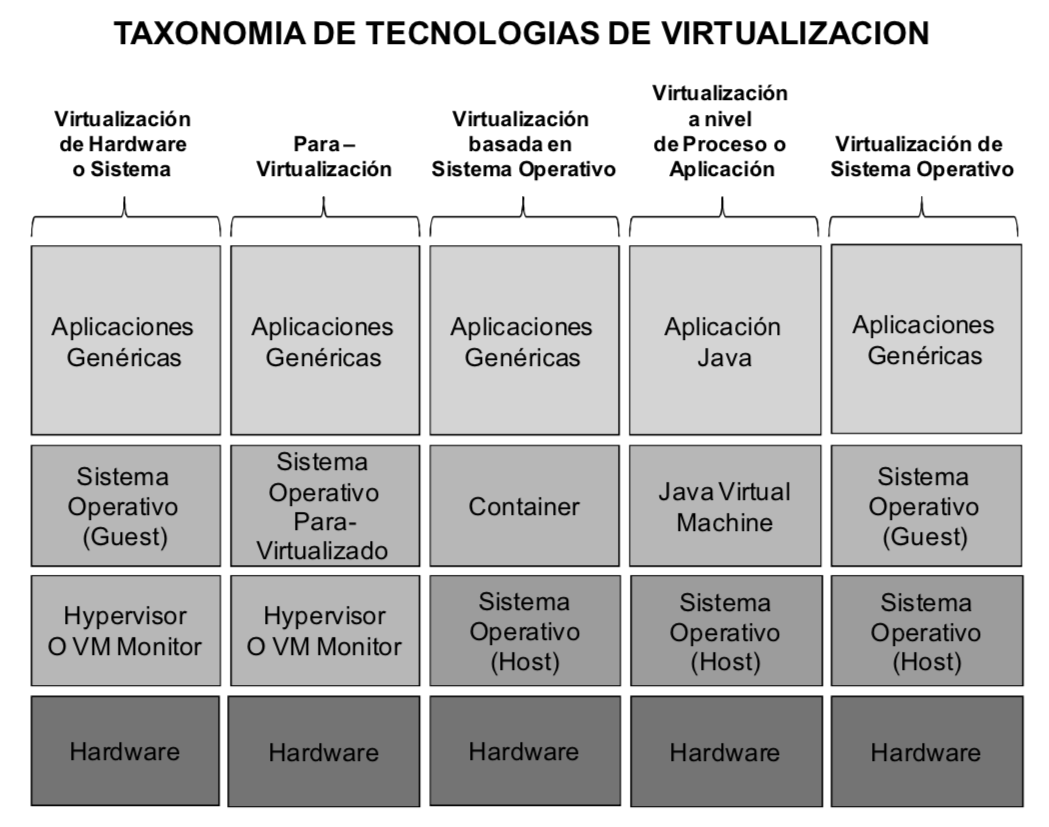
\includegraphics[width=0.8 \linewidth]{Pictures/taxonomiaPessolani.png}
	\vspace{-0.2cm}
	\caption{Taxonomía de máquinas virtuales propuesta por Pessolani y otros en 2012\footnotemark[8]{}}
	\label{fig:taxonomiaPessolani}
\end{figure}

\footnotetext[8]{Figura basada en el trabajo \textit{Sistema de virtualización con recursos distribuidos } de Pablo Pessolani, Toni Cortes, Silvio Gonnet y Fernando Tinetti, en 2005.}

El presente trabajo utiliza como base conceptual la taxonomía de tecnologías de virtualización propuesta por \textcite{Pessolani2012}. Esta taxonomía posee cinco categorías principales como son:\textit{virtualización de hardware o sistema}, \textit{para-virtualización}, \textit{virtualización basada en sistema operativo}, \textit{virtualización a nivel de proceso o aplicación} y finalmente \textit{virtualización de sistema operativo}. (Ver figura \ref{fig:taxonomiaPessolani}). Adicionalmente, también se muestran capas por cada categoría, las cuales sugieren un nivel en el cuál tiene lugar cada tipo de virtualización. A continuación, se describen las categorías de esta taxonomía:\\


\subsubsection{Virtualización de Hardware o Sistema}
Esta categoría se caracteriza por utilizar un hipervisor \textit{Tipo 1} directamente sobre el hardware (\textit{bare-metal}) y a partir de él, se ubican las VMs con sus respectivos sistemas operativos \textit{guest} (estos sistemas no logran percibir la condición de virtualización), los cuales soportan a su vez las aplicaciones particulares de los usuarios \parencite{Pessolani2012}.\\

Esta técnica de virtualización es también llamada \textit{Virtualización completa} y con relación a la arquitectura x86, está basada en la combinación de técnicas de traducción binaria y ejecución directa. Este enfoque busca traducir el código del kernel del sistema operativo \textit{guest}, para reemplazar las instrucciones no virutalizables con unas nuevas que tengan efecto en el hardware virtual\parencite{VMware2008}. 

\subsubsection{Para-Virtualización}
Esta categoría tiene la distribución de sus elementos similar a la \textit{virtualización de hardware o sistema} y también utiliza un hipervisor \textit{Tipo 1}, pero en este caso el sistema operativo \textit{guest} se considera que está \textit{Para-virtualizado}, esto es que ha sido modificado para tener conocimiento del hecho de estar virtualizado y de esta manera sacar provecho de esa situación y en consecuencia obtener un mejor rendimiento. \parencite{Pessolani2012}\\

La palabra ``Para'' viene del Griego y significa ``al lado de''. En este contexto entonces signfica ``al lado de la virtualización''. La \textit{paravirtualización} se refiere a la comunicación entre el sistema operativo \textit{guest} y el hipervisor para mejorar el desempeño y la eficiencia. Esta técnica de virtualización también es conocida como \textit{Virtualización asistida por el sistema operativo} \parencite{VMware2008}.



\subsubsection{Virtualización basada en Sistema Operativo}
Esta categoría, a diferencia de las anteriores no utiliza un hipervisor y en contraste, se basa en la utilización de espacios de trabajo independientes llamados \textit{contenedores}, los cuales están basados en el sistema operativo \textit{host}. Estos contenedores permiten la ejecución de aplicaciones genéricas de forma independiente.\\

\subsubsection{Virtualización a nivel de proceso o Aplicación}
Este tipo de virtualización utiliza un proceso  o aplicación sobre el sistema operativo para brindar una máquina virtual que permita la ejecución de procesos basados en esa máquina, por ejemplo JVM y las aplicaciones Java respectivamente. \\ 

\subsubsection{Virtualización de Sistema Operativo}
Este tipo de virtualización necesita un sistema operativo \textit{host} el cual lleva a cabo las funciones de un hipervisor para soportar los sistemas operativos \textit{guests},  que a su vez tienen sus propias aplicaciones completamente independientes, por ejemplo \textit{User Mode Linux} \parencite{Dike2006}  y \textit{Minix Over Linux} \parencite{Pessolani2012}.